\documentclass[border=10pt]{standalone}

\usepackage{tikz}
\usepackage{tikzsymbols}
\usetikzlibrary{calc,patterns,shapes.geometric}

\def\centerarc[#1](#2)(#3:#4:#5){\draw[#1] ($(#2)+({#5*cos(#3)},{#5*sin(#3)})$) arc (#3:#4:#5);}

\begin{document}
	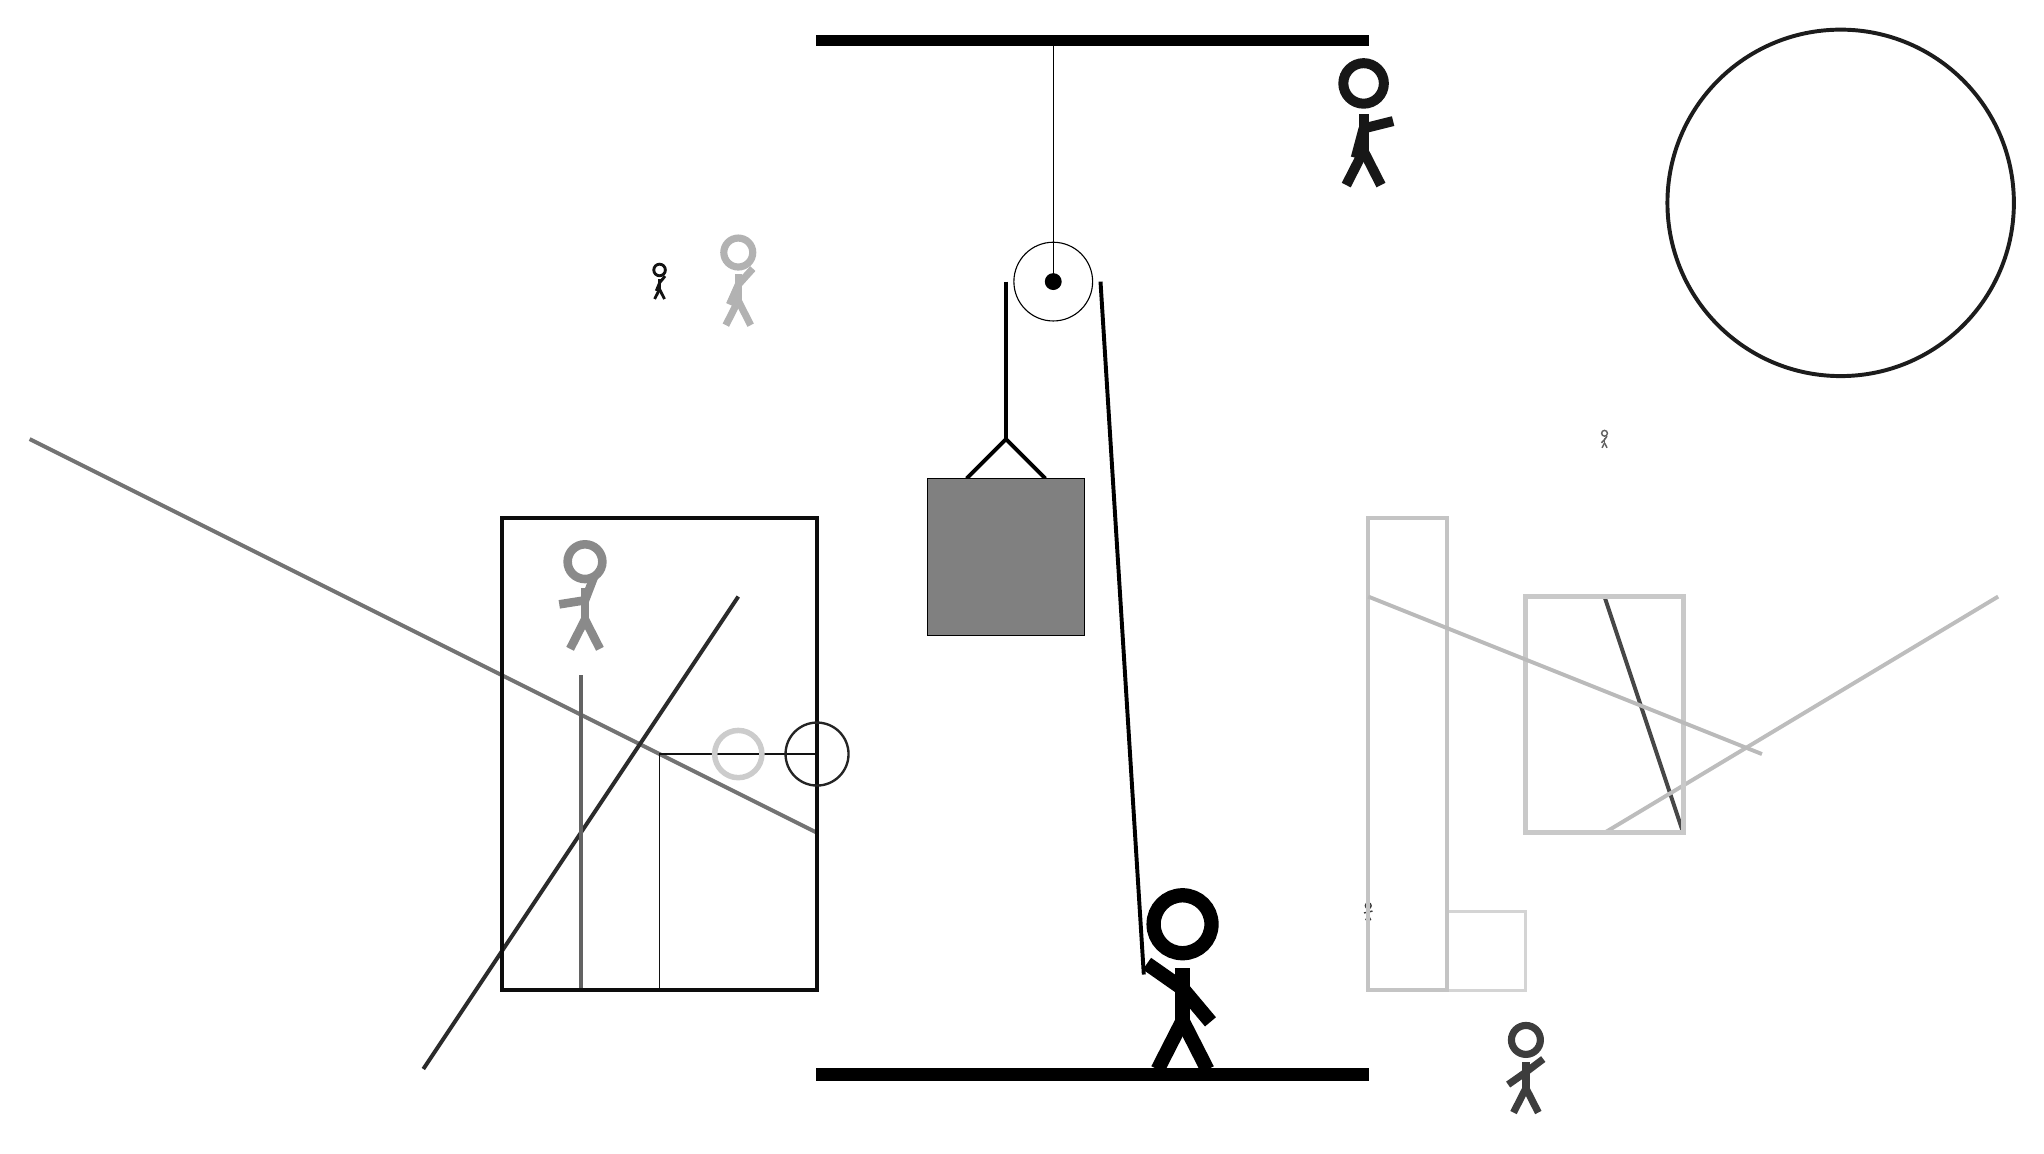
\begin{tikzpicture}
		%%%%% START %%%%%
		
		\draw[fill=black] (-2, 10) rectangle (5, 10.125);
		
		\draw (1, 7) circle (0.5);
		\draw[fill=black] (1, 7) circle (0.1);
		\draw (1, 10) -- (1, 7);
		
		\draw[line width=0.5mm] (-0.1, 4.5) -- (0.4, 5.0) -- (0.9, 4.5);
		\draw[fill=black!50] (-0.6, 4.5) rectangle (1.4, 2.5);
		
		\draw [line width=0.5mm, color=black!89](11, 8) circle (2.2);
		
		\draw[line width=0.5mm, color=black!72](8, 3) -- (9, 0);
		\draw[line width=0.5mm, color=black!26](8, 0) -- (13, 3);
		\node[line width=0.2mm, color=black!46] at (-5, 3) {\Strichmaxerl[6][9][69]};
		\node[line width=0.7mm, color=black!76] at (7, -3) {\Strichmaxerl[5][35][37]};
		
		\node[line width=0.7mm, color=black!62] at (8, 5) {\Strichmaxerl[1][45][55]};
		\draw[line width=0.5mm, color=black!55](-2, 0) -- (-12, 5);
		\node[line width=0.5mm, color=black!30] at (-3, 7) {\Strichmaxerl[5][66][48]};
		\node[line width=0.2mm, color=black!76] at (5, -1) {\Strichmaxerl[1][10][15]};
		
		\draw[line width=0.4mm, color=black!17] (7, -1) rectangle (6, -2);
		
		\draw[line width=0.5mm, color=black!83](-7, -3) -- (-3, 3);
		\draw[line width=0.2mm, color=black!93] (-2, 1) rectangle (-4, -2);
		\draw[line width=0.5mm, color=black!23] (5, 4) rectangle (6, -2);
		
		\draw[line width=0.5mm, color=black!61](-5, 2) -- (-5, -2);
		\draw[line width=0.6mm, color=black!21] (7, 3) rectangle (9, 0);
		\draw[line width=0.5mm, color=black!95] (-2, -2) rectangle (-6, 4);
		\draw [line width=0.7mm, color=black!20](-3, 1) circle (0.3);
		\draw[line width=0.5mm, color=black!27](5, 3) -- (10, 1);
		\draw [line width=0.3mm, color=black!86](-2, 1) circle (0.4);
		
		\node[line width=0.3mm, color=black!93] at (-4, 7) {\Strichmaxerl[2][68][51]};
		\node[line width=0.7mm, color=black!91] at (5, 9) {\Strichmaxerl[7][75][14]};
		
		
		\draw[line width=0.5mm] (0.4, 7) -- (0.4, 5.0);
		\centerarc[line width=0.5mm](1, 7)(0:180:0.6);
		\draw[line width=0.5mm](1.6, 7) -- (2.15, -1.8);
		
		\node at (2.6, -1.9) {\Strichmaxerl[10][-35][-50]};
		
		\draw[fill=black] (-2, -3) rectangle (5, -3.15);
		
		%%%%% END %%%%%
	\end{tikzpicture}
\end{document}